%!TEX root = ../../report.tex
\section{Content-based recommender systems}
\label{sec:content}
The overall reason to implement a Content-based recommender system is basically the same as for other recommender systems; to deliver a list of recommendations that statistically will be seen as valuable to the user. Where it differentiates itself from others is in the way these recommendations are generated.\newline 

A content-based recommender system will try to recommend items to the user similar to items that this user has interacted with in the past. In other words, the way the content-based recommender system approaches the recommendation process, is by analyzing previous items preferred by the user. From this information the user's interests are extracted and these will then be compared with items contained in the system.\newline
The system will then return items that are seen as relevant for the user, based on his interests. 

\subsection{The Components}
In this section we will describe the different components which represents the content-based recommender system. In the previous section we explained that it produces the recommendations in relation to the user's preferences, then by comparing these preferences with the items contained in the system, and finally choosing and presenting the recommended items to the user. \newline
There are three main steps used in this recommendation process, which are described as follows; content analysis, profile learning, and filtering. Figure \ref{contentdescription} illustrates the process and can be used as a reference to better comprehend some of the steps which are further explained below.

\begin{figure}[H]
\centering
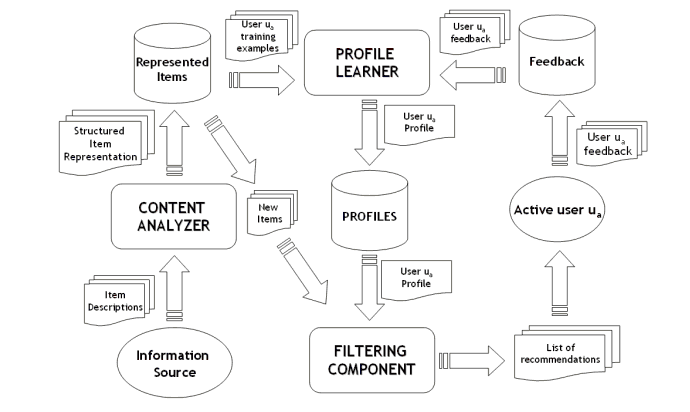
\includegraphics[width=90mm]{Pictures/contentdescription.png}
\caption{source: http://pyevolve.sourceforge.net/wordpress/?p=2497}
\label{contentdescription}
\end{figure}
\begin{itemize}
	\item \textbf{Content analyzer:}
	The main responsibility of the content analyzer is to represent data (items, web pages, articles, documents, etc.) in such a way that it can be used by the next processing steps. This is done by shifting the content representation from its original form(usually text) to a form, represented as vectors, which is usable by the filtering compontent.
	
	\item \textbf{Profile learner:} This module collects and utilizes the relevant information that has been analyzed and altered into a usable format by the content analyzer. In this case, relevant information is data which represents the users preferences. The profile learner aspires to put this information in order and then use this ordered data to create the user profiles.
	
	\item \textbf{Filtering component:} This component receives items from the content analyzer and user profiles from the profile learner, both represented as vectors. The filtering component then compares the vector representing the user, with the vector representing the items, to compute and produce a list of recommendations. 
\end{itemize}

These three components work together to recommend items to the user via a series of steps, as illustrated on figure \ref{contentdescription}.\newline 
The first step of the process occurs when the content analyzer receives a number of item descriptions from an information source.These descriptions are analyzed to extract specific keywords from the unstructured text, to end up with a structured representation of the items.\newline
In parallel to the proces of the content analyzer, the profile learner starts building the user profiles. These profiles can be computed purely based on information from the information source, but can also come from system profiles that users have created. These system profiles can contain user feedback, which can be either implicit or explicit. Explicit feedback refers to when the user actively makes a decision, such as giving a rating for a specific item. Implicit feedback refers to when the user does not make any active involvement, and is captured by monitoring and analyzing the user's activities and behavior.\newline
The last step of the process in then for the filtering component to compare the user profiles from the profile learner with the items from the content analyzer. The filtering component produces a list of similarities between items and a specific user and prioritizes this list with the most similar items being in top.  

%During the profile learner step, the information is processed together with the represented items to predict the relevance of these in relation to the user. In some system a user can also create a profile where his or her areas of interest are directly provided, thus making the feedback part of optional relevance.\newline
%There are basically two types of relevant feedback, positive and negative. The positive feedback indicates features that the user are interested in, whereas the negative feedback is an indicator of features that have no interest to the user. \newline
%These types of feedback can be recorded with two different feedback techniques, namely implicit and explicit feedback. Explicit feedback refer to when the user actively makes a decision, such as giving a rating for a specific item. Implicit feedback refers to when the user does not make any active involvement, and is captured by monitoring and analyzing the user's activities and behavior.\newline
%The explicit feedback technique is the easiest way for the recommender system to make recommendations, because it gives a clear and actual indication of the users preferences. When speaking about the explicit kind of feedback, there are three main approaches: like or dislike, ratings, and comments on items.\newline
%The first option works as a binary scale where the user can either choose to like or dislike an item.The rating option gives the user a larger scale to rate an item on, for instance from 1-10, where 10 indicates the most-liked option. The last option presents the user with a set of text comments from other users in order to aid the user in the decision-making whether to buy or not buy a specific item.\newline

%All of the above mentioned steps will help the profile learner to create a more comprehensive overview of the users preferences. An advantage of the explicit feedback is that it simplifies the interpretation process of the recommender system for the items in question. A disadvantage are that the user is required to make an active choice, hence incurring a cognitive load on the user. The implicit feedback is centered around actions that do not require direct user involvement on a cognitive level, but more on their actions in relation to the items in question, such as saving, discarding, bookmarking, etc.\newline

%In order for the recommender system to create a user profile, it is needed by the system to first create something called a training set consisting some of the current items in the system. This training set is then used by the profile learner to match up against the user's preferences to build a solid foundation for the user profile. The training set of recommendations is updated on a regular basis in order to keep the recommendations as close to the users current preferences as possible. $$$$This is of particular importance because a users preferences are most likely to be in a dynamic state of change over time$$$.\newline
%Future items added to the system will be matched against the users item preferences via the filtering component and, if there is a match, these items will be added to the training set and shown as recommendations to the user. \\

In the next section we will discuss how the similarity of items in relation to user profiles are computed.

\subsection{Vector Space Model}
The way most content-based recommender systems defines the relevance of an item is by the Vector Space Model (VSM), which is a representation of text documents in the form of vectors. Each of the documents is represented by a vector in a \(n\)-dimensional space where \(n\) represents the number of keywords from that particular document that matches the overall list of keywords.\newline
When using VSM to represent the weight of keywords in documents, there are two things that are important: 1) Giving a weight to the keyword, indicating the importance of the keyword in relation to the document, where the keyword is found in and 2) measure the importance of the document in relation to all the other documents contained in the system. A computational scheme which can be used for this is TF-IDF. \newline

\textbf{TF-IDF} stands for Term Frequency / Inverse Document Frequency and is used to generate a weight for a specific keyword \(t_{k}\) in a specific document \(d_{j}\), in relation to all documents. TF-IDF is divided into two parts.\newline
The first part is Term Frequency which counts the number of occurrences of a specific keyword \(t_{k}\) in the document \(d_{j}\), and gives this keyword a weight of importance in relation to the keyword in the document with the maximum number of occurrences. %TF can also be divided by document length, to ensure that a book which have the keyword in it eight times, is not favored over a short document which contains the same keyword four times, because a short document with four occurrences might be of a bigger value to the user than an entire book with only eight occurrences.\newline
The second part is Inverse Document Frequency, which analyzes how many documents contains this keyword. The formulas for these calculations will be explained further below in this section. \newline
If a keyword happens to be noted often in several documents, this specific keyword will not be given too much weight, because the system sees it as common. On the other hand, if a keyword occurs frequently in a few documents, but infrequently in all other documents in the system, this keyword will achieve a higher weight.\newline

The document vector is generated by checking the keywords contained within the document. These keywords are given a weight in relation to their significance. The document vectors consists of the values of each keyword. 

The user vector is generated by checking the keywords for the documents that the user has previously interacted with (bought, viewed, tagged, etc.).\newline
The vectors of the document profile and the user profile are compared by the system by calculating the angle between the vectors. The smaller the angle, the more aligned the document is with the user interests. In many recommender systems, instead of the angle, the cosine to the angle is used, which gives a value from 0 to 1, 1 being the perfect match.\newline

To understand the concept of the vector weighting we imagine that we have a content space, with as many dimensions as there a keywords in the system. Each of the documents and user profiles in the system are represented by a vector in this content space.\newline

There are several ways where a vector can be computed. Here we will outline the three most common ways.
1) A vector can represent a fact (true/false) and can be computed simply by using a boolean value. An example of this can be whether a specific keyword is used in a specific document. A boolean would be used here because it is not possible to give this vector a further notion of intensity.\newline
2) Another way to compute a vector is by counting the number of keyword occurrences in a document, which can help give a bigger notion of intensity for the vector.\newline
3) Use the TF-IDF which implements both of the above mentioned methods, because it gives us a notion of intensity in a document along with a notion of distinctiveness for the individual vector. This approach is described below.\newline

TF calculates a value for a specific keyword in relation to how many times it occur in the specific document \(d_{j}\) and how many times the most frequently used keyword \(k\) occur.
%TF
\[
	\text{TF}(t_{k},d_{j}) = \frac{f_{k,j}}{max_{z}f_{z,j}}
\]

The TF-IDF approach adds an extra layer to the TF, by further calculating the keyword occurrences in relation to all documents in the system.
%TF-IDF
\[
	\text{TF-IDF}(t_{k},d_{j}) = \text{TF}(t_{k},d_{j}) * log{\frac{N}{n_{k}}}
\]

Cosine normalization is used to scale all the weights in the calculation to give them a value between 0 and 1.
%cosine normalization
\[
	w_{k,j} = \frac{\text{TF-IDF}(t_{k},d_{j})}{\sqrt{\sum_{s=1}^{|T|} \text{TF-IDF}(t_{s}, d_{j})^2}}
\]

The cosine similarity is used to indicate the similarity between two vectors, which then can be used to predict whether a user will be interested in a particular item or not. The result is a value between 0 and 1, where 1 indicates a big similarity between the items.

%cosine similarity
\[
	sim({d_{i},d_{j}}) = \frac{\sum_{k}w_{ki}*w_{kj}^2}{\sqrt{\sum_{k}w_{ki}^2}*\sqrt{\sum_{k}w_{kj}^2}}
\]


%While some of the challenges of recommender systems is to figure out the right weights and factors to use to compute the recommendations for the users, most of the basic recommender system does not handle interdependencies, since it most often are outside the scope of the systems work area.\newline
%An example of an interdependency could be from the movie world where a user might like comedies with violence, and historical documentaries, but do not like historical comedies or violent documentaries (or likes Sean Connery in action movies and Owen Wilson in comedies, but not vice versa). \newline
%Since we can state that the vectors in this case would be comedies, violence, historical, and documentaries, the system in its simplicity will have no chance of interpreting the relationship of the users actual preferences, since the system does not have the notion of multiplying different dimensions together. If taking interdependencies into account is a necessity, it is possible to implement this by using a method called LSI/SVD, which stands for Latent Semantic Indexing/Singular Value Decomposition. LSI/SVD identifies associations and patterns between terms and keywords in a text, and adds an extra dimension to the precision with which it is possible to recommend objects to users. LSI/SVD lies beyond the scope of this report and we will not go any further into the functionality of it.\newline

The methods described in this section are essential for a content-based recommender system because they are the foundation on which the recommendations are made.

\subsection{Advantages and disadvantages}
When looking at recommender systems from a content-based systems point of view there are several advantages over a recommender system in a collaborative-based form.\newline

The three main areas of advantage are: User independence, transparency, and new items.\newline
The \textbf{user independence} shows itself in that the content-based recommendations are solely based on the active user's own preferences and does not rely on the interaction with others.\newline
The content-based recommendations are \textbf{transparent} in the way that all its recommendations are clearly based on the users list of preferences.\newline
The advantage of a content-based recommender system in regards to \textbf{new items} that enters the system, is that these items will not need to be rated prior to being recommended to the users. Here, the only dependency is whether the item is similar enough to the individual users preferences.\newline

As well as the above mentioned advantages, a content-based recommender system also has some disadvantages. The three main areas here are: Limited content analysis, over-specialization, and new users.\newline

The \textbf{limited content} analysis revolves around the fact that content-based recommender systems most often are dependent on domain knowledge. An example of this could be for a movie recommendation. Here, the recommender system would need to know the actors, director, genre, and alike. If the content analyzer does not find this information within the provided data, then it will be virtually impossible for the recommender system to distinguish between items correlating with the user preferences and items that are of no interest at all.\newline

The \textbf{over-specialization} is that the user will never be recommended any items in a positive unexpected manner. What is meant by this is that the user's personal area of preferences might be somewhat wider than the area of the current information held in the User Profile, but because the recommended items for the individual user is based on a similarity with items previously interacted with by the user, there will never be a recommendation deviating from this.\newline
The \textbf{new user disadvantage} can be sort of a predicament for the recommender system. The issue here is that to give the new user a fair recommendation based on user interests and preferences, the user will need to have interacted with a certain amount of items for the filtering component to compare with. When the new user first create his or her account, the recommender system is somewhat forced to either recommend a set of random items or recommend what the average user would be recommended. In most recommender systems the latter is the solution of choice.

